%%
%% Copyright 2007, 2008, 2009 Elsevier Ltd
%%
%% This file is part of the 'Elsarticle Bundle'.
%% ---------------------------------------------
%%
%% It may be distributed under the conditions of the LaTeX Project Public
%% License, either version 1.2 of this license or (at your option) any
%% later version.  The latest version of this license is in
%%    http://www.latex-project.org/lppl.txt
%% and version 1.2 or later is part of all distributions of LaTeX
%% version 1999/12/01 or later.
%%
%% The list of all files belonging to the 'Elsarticle Bundle' is
%% given in the file `manifest.txt'.
%%

%% Template article for Elsevier's document class `elsarticle'
%% with numbered style bibliographic references
%% SP 2008/03/01
%%
%%
%%
%% $Id: elsarticle-template-num.tex 4 2009-10-24 08:22:58Z rishi $
%%
%%
%\documentclass[preprint,12pt]{elsarticle}
\documentclass[5p]{elsarticle}

%% Use the option review to obtain double line spacing
%% \documentclass[preprint,review,12pt]{elsarticle}

%% Use the options 1p,twocolumn; 3p; 3p,twocolumn; 5p; or 5p,twocolumn
%% for a journal layout:
%% \documentclass[final,1p,times]{elsarticle}
%% \documentclass[final,1p,times,twocolumn]{elsarticle}
%% \documentclass[final,3p,times]{elsarticle}
%% \documentclass[final,3p,times,twocolumn]{elsarticle}
%% \documentclass[final,5p,times]{elsarticle}
%% \documentclass[final,5p,times,twocolumn]{elsarticle}

%% if you use PostScript figures in your article
%% use the graphics package for simple commands
%% \usepackage{graphics}
%% or use the graphicx package for more complicated commands
%% \usepackage{graphicx}
%% or use the epsfig package if you prefer to use the old commands
%% \usepackage{epsfig}

%% The amssymb package provides various useful mathematical symbols
\usepackage{amssymb}
%% The amsthm package provides extended theorem environments
%% \usepackage{amsthm}

%% The lineno packages adds line numbers. Start line numbering with
%% \begin{linenumbers}, end it with \end{linenumbers}. Or switch it on
%% for the whole article with \linenumbers after \end{frontmatter}.
%% \usepackage{lineno}

%% natbib.sty is loaded by default. However, natbib options can be
%% provided with \biboptions{...} command. Following options are
%% valid:

%%   round  -  round parentheses are used (default)
%%   square -  square brackets are used   [option]
%%   curly  -  curly braces are used      {option}
%%   angle  -  angle brackets are used    <option>
%%   semicolon  -  multiple citations separated by semi-colon
%%   colon  - same as semicolon, an earlier confusion
%%   comma  -  separated by comma
%%   numbers-  selects numerical citations
%%   super  -  numerical citations as superscripts
%%   sort   -  sorts multiple citations according to order in ref. list
%%   sort&compress   -  like sort, but also compresses numerical citations
%%   compress - compresses without sorting
%%
%% \biboptions{comma,round}

% \biboptions{}


\journal{DFRWS 2012}

\begin{document}

\begin{frontmatter}

%% Title, authors and addresses

%% use the tnoteref command within \title for footnotes;
%% use the tnotetext command for the associated footnote;
%% use the fnref command within \author or \address for footnotes;
%% use the fntext command for the associated footnote;
%% use the corref command within \author for corresponding author footnotes;
%% use the cortext command for the associated footnote;
%% use the ead command for the email address,
%% and the form \ead[url] for the home page:
%%
%% \title{Title\tnoteref{label1}}
%% \tnotetext[label1]{}
%% \author{Name\corref{cor1}\fnref{label2}}
%% \ead{email address}
%% \ead[url]{home page}
%% \fntext[label2]{}
%% \cortext[cor1]{}
%% \address{Address\fnref{label3}}
%% \fntext[label3]{}

\title{Using NLP Techniques for File Fragment Classification}

%% use optional labels to link authors explicitly to addresses:
%% \author[label1,label2]{<author name>}
%% \address[label1]{<address>}
%% \address[label2]{<address>}

%\author{Simran Fitzgerald, George Mathews, Colin Morris and Oles Zhulyn}

\address{}

\begin{abstract}
The classification of file fragments is an important problem in digital forensics. The literature does not include comprehensive work on applying machine learning techniques to this problem. In this work, we explore the use of techniques from natural language processing to classify file fragments. We took a supervised learning approach, based on the use of support vector machines combined with the bag-of-words model, where text documents are represented as unordered bags of words. This technique has been repeatedly shown to be effective and robust in classifying text documents (e.g., in distinguishing positive movie reviews from negative ones).

In our approach, we represent file fragments as ``bags of bytes'' with feature vectors consisting of unigram and bigram counts, as well as other statistical measurements (including entropy and others). We made use of the publicly available Garfinkel data corpus to generate file fragments for training and testing. We ran a series of experiments, and found that this approach is effective in this domain as well.
\end{abstract}

\begin{keyword}
%% keywords here, in the form: keyword \sep keyword
file fragment classification \sep machine learning \sep support vector machine \sep digital forensics

%% MSC codes here, in the form: \MSC code \sep code
%% or \MSC[2008] code \sep code (2000 is the default)

\end{keyword}

\end{frontmatter}

%%
%% Start line numbering here if you want
%%
% \linenumbers

%% main text
\section{Introduction}
\label{Section:Introduction}
The classification of file fragments is an important problem in digital forensics, particularly for the purpose of carving fragmented files. Files that are not stored contiguously on the hard drive must be carefully reconstructed from fragments based on their content during file carving. Because the search space for fragments belonging to a particular file is so large, it is essential to have an automated method for distinguishing whether a fragment potentially belongs to a file or not. For example, a fragment from a plain-text file (e.g. \texttt{txt}) certainly does not belong to a compressed image file (e.g. \texttt{jpg}). Garfinkel \cite{Garfinkel07} observes that although the fragmentation of files is relatively rare on today's file systems, the files of interest in forensic investigations are more likely to be fragmented than other files. For example, large files that have been modified numerous times over a long period of time on a hard drive that is filled near capacity, will likely exhibit fragmentation. In this work, we explore the application of machine learning techniques from natural language processing to the problem of file fragment classification.

Classification is a standard machine learning problem. There has been work done on applying machine learning techniques to the problem of file fragment classification \cite{Axelsson10, Conti10, Li10, Veenman07}. However, the body of work in the literature is not exhaustive. Our contribution to this problem, is the application of supervised machine learning techniques used in natural language processing.

In previous work, the histograms of the bytes within file fragments are used for classification \cite{Li05, Li10, Stolfo05, Veenman07}. In natural language processing, this kind of approach is called the ``bag-of-words model'', where text documents are represented as unordered bags of words. The single word tokens are called unigrams, but tokens consisting of any fixed number of words can also be considered. Two word tokens are called bigrams, and bigram counts capture more information about the structure of the data being classified than do unigram counts alone. Combined with various machine learning techniques, this kind of approach has been repeatedly shown to be effective and robust in classifying text documents (e.g. in determining whether a piece of text has a positive or negative sentiment). In our approach, we consider the unigram and bigram counts of the bytes within file fragments, along with other statistical measurements, to generate feature vector representations of the file fragments, which we then classify based on 24 different file types using a support vector machine.

Support vector machines are supervised machine learning algorithms that are very effective for classification problems \cite{Li10}. During the training phase, a support vector machine partitions a high-dimensional space based on the points it contains that belong to known classes. File fragments can be represented in the high-dimensional space by being transformed into feature vectors. During the testing phase, file fragments of unknown types are transformed into feature vectors and are classified according to what partition they lie in in the high-dimensional space. We make use of the \texttt{libsvm} \cite{CC01a} library, which is the one of the most widely used implementations of support vector machines, to perform our experiments.

Most of the previous work on this problem exclusively uses private data sets, making it more difficult for other researchers to reproduce experimental results. We follow the example of Axelsson \cite{Axelsson10} and derive the data set we use for training and testing from the freely available corpus of forensics research data by Garfinkel et al. \cite{Garfinkel09} (the \texttt{govdocs1} data set described in Section 4 of the cited paper). We determined the most well-represented file types in the data set and selected 24 of them based on how well-known they are. For each of the 24 file types supported by our classifier, we downloaded files uniformly at random from the \texttt{govdocs1} data set such that we would have at least 10 files made up of at least 10000 512-byte fragments. From this, we uniformly at random selected 9000 fragments for each file type to create our data set. When generating the fragments, we omitted the first and last fragments of each file, as the first fragment frequently contains header information that identifies the file type, and the last fragment might not be 512 bytes in length.

Our experiments consisted of selecting uniformly at random the same fixed number of file fragments for each of the 24 file types. We partitioned the resulting set of file fragments into a training set and a testing set in a 9-to-1 ratio, such that no file had file fragments appearing in both sets. We trained the support vector machine on the training set and tested it on the testing set. The results we got are very promising, outperforming comparable results from previous work.

The paper is organized as follows. In Section \ref{Section:RelatedWork}, we provide a brief overview of related work done in this area. In Section \ref{Section:ExperimentalSetup}, we describe our experimental setup, which includes how we generated the data set we used in training and testing, as well as details about the features we used in our feature vectors. In Section \ref{Section:Results}, we present our results. We conclude and suggest future directions for this work in Section \ref{Section:ConclusionAndFutureWork}.

\section{Related work}
\label{Section:RelatedWork}
Previous work that explores the application of machine learning techniques to the problem of file fragment classification appears in the literature.

Calhoun and Coles \cite{Calhoun08} considered only four file types (namely, \texttt{jpg}, \texttt{bmp}, \texttt{gif}, and \texttt{pdf}). For each pair of these file types, they used linear discriminant analysis \cite{Fisher36} (which is used to find linear combinations of features to characterize or separate objects between classes) in order to classify a file fragment as having one type or the other. The features they considered were various statistical measurements, including Shannon entropy \cite{Shannon48} and frequency of ASCII codes. They achieved fairly good accuracy (88.3\%). However, since they classified fragments based on only four file types on a pairwise basis, it is not clear how well this technique would generalize to a real-world application, where a given file fragment is not known to belong to a file of only two possible types.

Axelsson \cite{Axelsson10} considered 28 different file types and applied the k-nearest-neighbors classification technique with nearest compression distance as the distance metric between file fragments. The file fragment data was generated from the freely available \texttt{govdocs1} corpus by Garfinkel et al. \cite{Garfinkel09}. Axelsson's experiments consisted of ten trials. In each trial, 10 files were selected at random (with the types of the files uniformly distributed) and 14 512-byte fragments were extracted at random from each of them. The fragments were then classified against a data set of approximately 3000 file fragments with known types. The average classification accuracy was around 34\%, with higher accuracy being achieved for file fragments with lower entropy.

Conti et al. \cite{Conti10} made use of a private data set of 14000 1024-byte binary fragments which they characterized by vectors of statistical measurements (namely, Shannon entropy, Hamming weight, Chi-square goodness-of-fit, and mean byte value). They classified each of these vectors against the remaining 13999 using k-nearest-neighbors with Euclidean distance as the distance metric. They achieved 98.55\% classification accuracy for Random/Compressed/Encrypted fragments, 100\% for Base64 Encoded fragments, 100\% for Unencoded fragments, 96.7\% for Machine Code (ELF and PE) fragments, 98.7\% for Text fragments, and 82.5\% for Bitmap fragments. However, the classifier did not perform as well when applied to real-world binary data, especially when it contained fragments of ``a previously unstudied primitive type, even one with a closely related structure''. They also classified the fragments according to types of a very coarse granularity.

Li et al. \cite{Li05} used the histogram of the byte values (unigram counts) of the prefix of a file (along with other portions of the file) in order to classify its type. They first collected a private data set of files across 8 different file types, and applied the k-means clustering algorithm to generate models for each file type (i.e. the centroids for the histograms of the files of that type). They achieved very good classification accuracy. However, this approach explicitly relies on the header information contained in each file, and hence, is not applicable to most file fragments which do not contain this information.

Veenman \cite{Veenman07} used the histogram of the byte values (unigram counts), the Shannon entropy, and the algorithmic or Kolmogorov complexity \cite{Kolmogorov65, Lempel76} as features for linear discriminant analysis to classify file fragments that were 4096 bytes in size. Veenman used a large private data set consisting of between 3000 and 20000 fragments per file type, for 11 file types. Veenman achieved an average classification accuracy of 45\%.

Li et al. \cite{Li10} used a support vector machine with feature vectors based on the histogram of the byte values (unigram counts) to classify high entropy file fragments that were 4096 bytes in size. They used a private data set consisting of 880 \texttt{jpg} images, 880 \texttt{mp3} music files, 880 \texttt{pdf} documents, and 880 \texttt{dll} files for training and testing the support vector machine. They achieved an average classification accuracy of 81.5\%. It is likely that the large file fragment size made the classification task easier. However, in the absence of file system information in a real-world situation, a large file fragment size cannot be assumed. Furthermore, this work does not take into consideration other high entropy file types that might be of interest (such as \texttt{zip} or \texttt{gz} compressed files). Some differences between the work of Li et al. and ours are as follows. The data set we used is derived from a freely available corpus, making it easier to reproduce our work, unlike Li et al. We considered a file fragment size which can be safely assumed when no file system information is available \cite{Axelsson10}, unlike Li et al. Our classifier supports a much larger variety of file types, including both low and high entropy ones, unlike Li et al.

\section{Experimental setup}
\label{Section:ExperimentalSetup}

\subsection{Data Set}
\label{Subsection:DataSet}

\begin{figure}[t!]
\centering
% TODO FIX
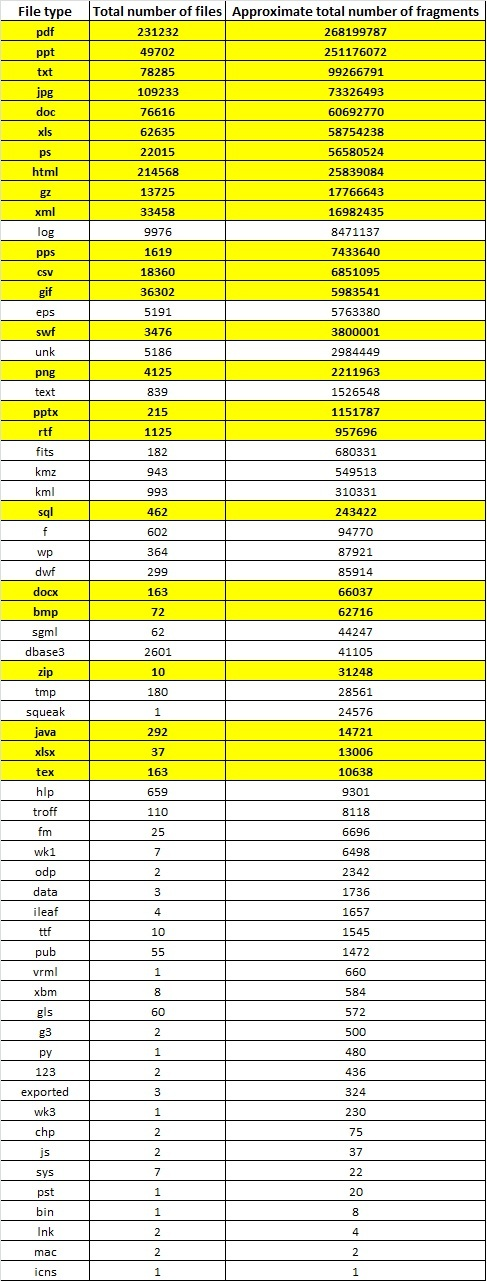
\includegraphics[height=590pt]{gov_docs_dataset.ps}
\caption{\textit{Statistics on the \texttt{govdocs1} data set. The highlighted file types are the ones we used for our classifier.}\label{fig:govdocs1DataSet}}
\end{figure}

The data set we used for training and testing is derived from the freely available corpus of forensics research data by Garfinkel et al. \cite{Garfinkel09} (the \texttt{govdocs1} data set described in Section 4 of the cited paper). We determined the most well-represented file types in the data set and selected 24 of them based on how well-known they are to us (see Figure \ref{fig:govdocs1DataSet}). The first of these criteria ensured that we acquired a good variety of file fragment data for each file type. The second of these criteria is not a rigorous one. Although we aimed to get a good representation of file types that are likely to be of forensic interest, a rigorous methodology for selecting the most appropriate file types is outside the scope of this paper. Nevertheless, most of the file types we selected overlap with the ones selected by Axelsson \cite{Axelsson10} who made use of the same Garfinkel corpus to derive his data set.

After selecting the file types, we proceeded to download files uniformly at random from the \texttt{govdocs1} corpus such that we would have at least 10 files made up of at least 10000 512-byte fragments for each of the 24 file types. Because the files in the \texttt{govdocs1} corpus are of variable length, and files from different file types are not equally represented, it was necessary to download more than 10 files or files that altogether constituted more than 10000 fragments, for each of the file types, in order to meet both criteria. From this, we uniformly at random selected 9000 fragments for each file type to create our data set. When generating the fragments, we omitted the first and last fragments of each file, as the first fragment frequently contains header information that identifies the file type, and the last fragment might not be 512 bytes in length. Calhoun and Coles \cite{Calhoun08}, Conti et al. \cite{Conti10}, and Li et al. \cite{Li10} omit these fragments as well. This approach enabled us to generate a large data set of file fragments with an equal number of file fragments for each file type, and with each fragment being derived from a variety of files with the same type.

\subsection{Feature Vectors}
\label{Subsection:FeatureVectors}
During the training phase, a support vector machine partitions a high-dimensional space based on data points with known classes, with each partition corresponding to a class. In order to train a support vector machine on the file fragment data, it is necessary to represent each file fragment as a point in a high-dimensional space. We do this by transforming each file fragment into a vector of features. The features we used are described here.

There are 256 features which are the histogram of the byte values (i.e. the unigram counts) for the file fragment. The feature vectors in the work by Li et al. \cite{Li10} consist only of the unigram counts. Another $256^2$ features in our work are the histogram of the pairs of consecutive byte values (i.e. the bigram counts) for the file fragment.

We also have features for various statistical measurements. We have the Shannon entropy \cite{Shannon48} of the bigram counts. Conti et al. \cite{Conti10} considered the Shannon entropy of the unigram, bigram, and trigram counts, and found that the entropy of the bigram counts was effective for classifying file fragments. We made use of the Hamming weight (the total number of ones divided by the total number of bits in the file fragment) and the mean byte value features that appear in the paper by Conti et al. We also used the compressed length of the file fragment as a feature. We did this to approximate the algorithmic or Kolmogorov complexity of the file fragment, following Veenman \cite{Veenman07}. We compressed each file fragment with the \texttt{bzip2} algorithm \cite{Seward01}. We also used two features from natural language processing. We computed the average contiguity between bytes (i.e. the average distance between consecutive bytes) for each file fragment, which is defined as follows:

\begin{center}
 $\sum_{i=0}^{n=510}\frac{|fragment[i] - fragment[i+1]|}{511}$
\end{center}

{\noindent}where $fragment[i]$ is the $i^\textrm{\small th}$ byte of the file fragment. Last of all, we calculated the longest contiguous streak of repeating bytes for each file fragment.

\subsection{Experiments}
\label{Subsection:Experiments}
We ran three experiments. For each experiment, we selected uniformly at random file fragments for each of the 24 file types. The only difference between the three experiments was the upper limit on the number of file fragments for each file type that was selected (i.e. 1000, 2000, and 4000). During an experiment, the set of file fragments was partitioned into a training set and a testing set in a, roughly, 9-to-1 ratio. We ensured that no file had file fragments occurring in both the training set and the testing set. We then proceeded to train the support vector machine on the training set with default parameters and the linear kernel. Li et al. \cite{Li10} found that the linear kernel was the most effective when classifying file fragments represented by feature vectors consisting of the histogram of the byte values (unigram counts). Once a model was generated from the training data, we had the support vector machine attempt to classify the file fragments in the testing set. We repeated each of the three experiments ten times, each time selecting file fragments uniformly at random from our data set.

\section{Results}
\label{Section:Results}
\begin{figure}[t]
\centering
% TODO FIX
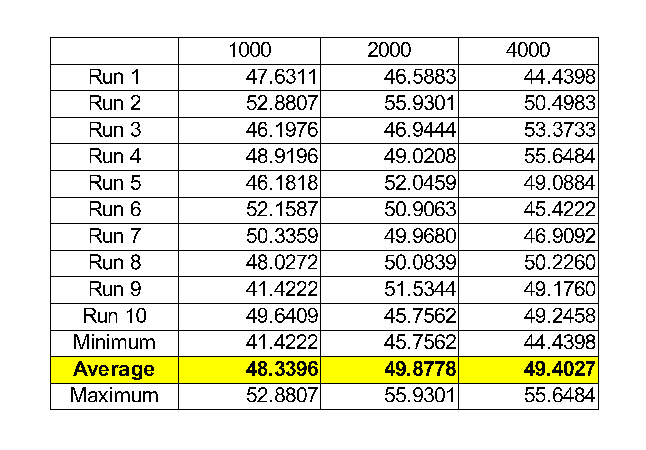
\includegraphics[width=3in]{results.ps}
\caption{\textit{Classification accuracy (in percent)}\label{fig:PredictionAccuracy}}
\end{figure}

\begin{figure*}[ht!]
\centering
% TODO FIX
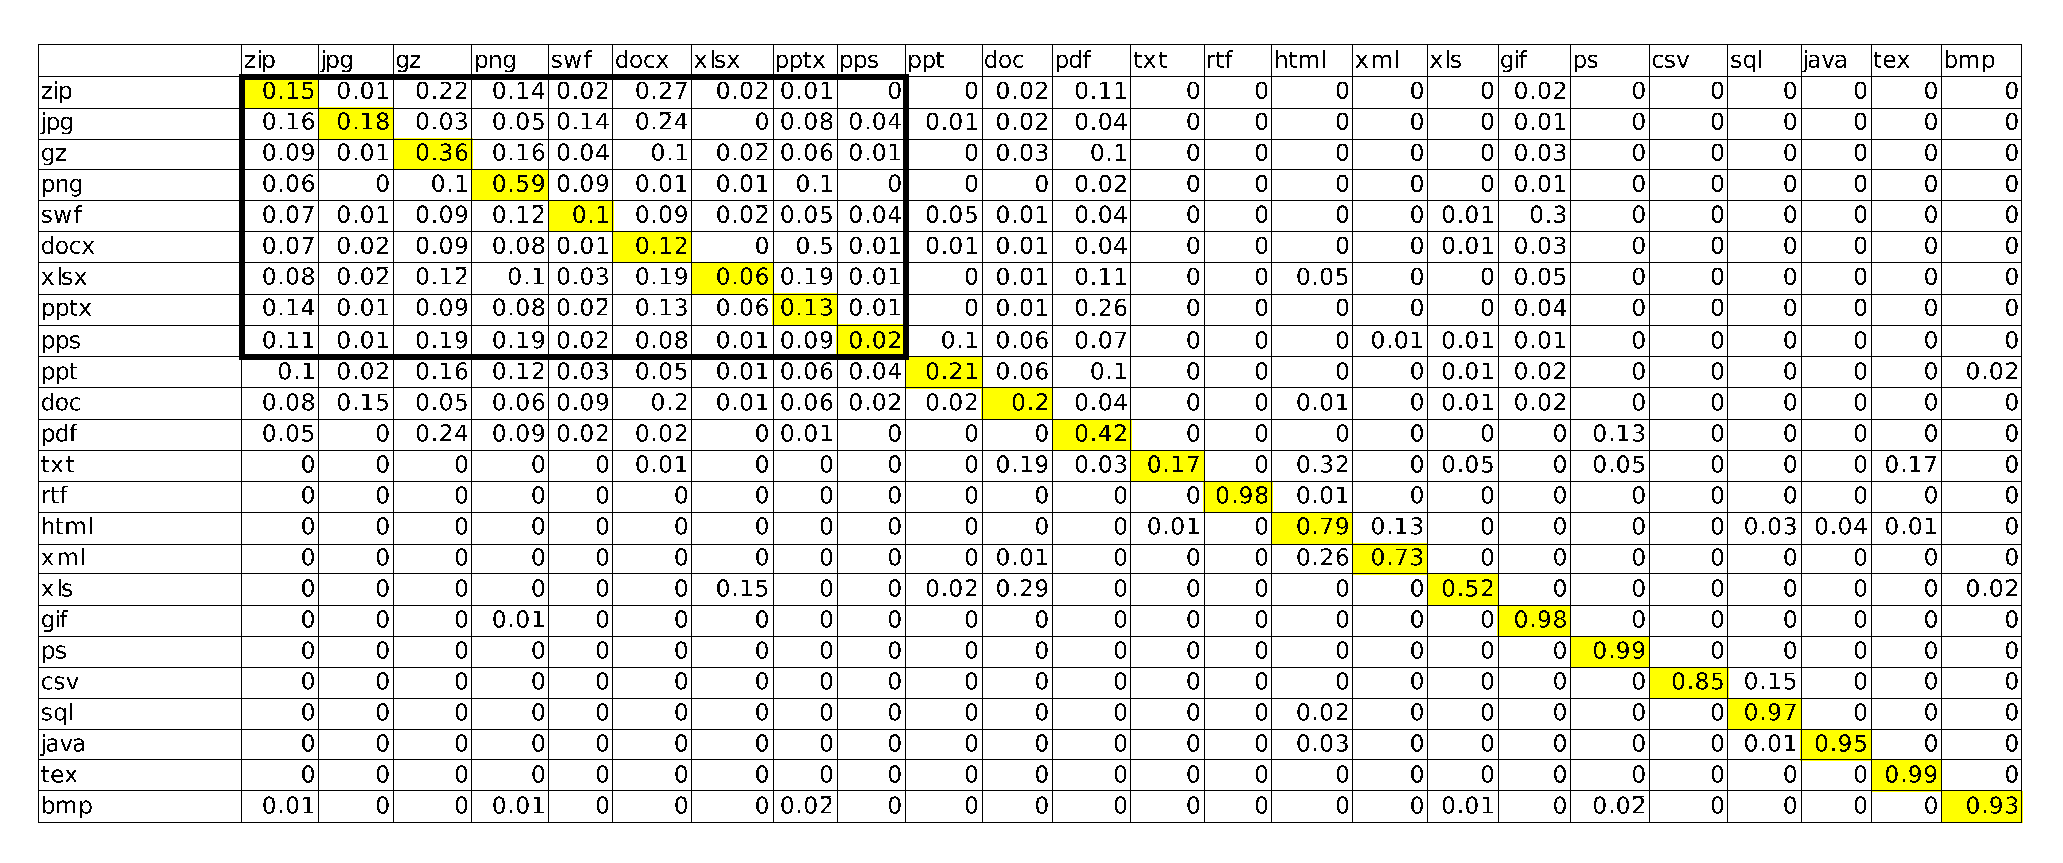
\includegraphics[width=7in]{confuseMatrix4k.ps}
\caption{\textit{Confusion matrix from one of the runs of the experiment that limited the number of file fragments per file type to 4000. The rows correspond to the actual file types and the columns correspond to what file types the file fragments were classified as. The file types in the top left correspond to high entropy files.}\label{fig:ConfusionMatrix4k}}
\end{figure*} 

After running the experiments, we found that our approach produced very good results. For the experiments that limited the number of file fragments per file type to 1000, we achieved an average prediction accuracy of 48.3396\% (with a minimum of 41.4222\% and a maximum of 52.8807\% for the ten runs). For the experiments that limited the number of file fragments per file type to 2000, we achieved an average prediction accuracy of 49.8778\% (with a minimum of 45.7562\% and a maximum of 55.9301\% for the ten runs). For the experiments that limited the number of file fragments per file type to 4000, we achieved an average prediction accuracy of 49.4027\% (with a minimum of 44.4398\% and a maximum of 55.6484\% for the ten runs). There was no significant improvement in the average prediction accuracy for the experiments that limited the number of file fragments per file type to 4000 over the ones that limited the number to 2000.

In terms of average prediction accuracy, our classifier has outperformed the most directly comparable classifiers in previous work. In particular, recall that Axelsson \cite{Axelsson10} achieved an average prediction accuracy of 34\% on 28 file types, and Veenman \cite{Veenman07} achieved an average prediction accuracy of 45\%, but only on 11 file types. Our classifier achieved an average prediction accuracy of 49.8778\% on 24 file types.

Our classifier did best on low entropy file fragments (e.g. plain-text files, uncompressed images, etc.), and worst on high entropy file fragments (e.g. compressed files, binary executables, etc.) (see Figure \ref{fig:ConfusionMatrix4k}). This reflects the findings in previous work (i.e. high entropy file fragments are harder to classify). In future work, the improvement of classification performance on high entropy file fragments should be investigated, such as through the use of the various machine learning boosting techniques.


\section{Conclusion and future work}
\label{Section:ConclusionAndFutureWork}
File fragment classification is an important problem in digital forensics. For this paper, we explored the application of supervised machine learning techniques from natural language processing to this problem. We generated a large data set of file fragments for 24 different file types, which we derived from the freely available \texttt{govdocs1} corpus by Garfinkel et al. \cite{Garfinkel09}. We represented each file fragment with a feature vector consisting of the unigram and bigram counts of bytes in the fragment, along with several other statistical measurements (such as entropy). Our file fragment classification approach consisted of using a support vector machine along with these feature vectors. We ran several experiments, and found this to be an effective approach, which outperformed comparable ones in the literature.

The results we got are promising, and several directions for future work on this project are apparent. For one, by scaling the feature vectors and finding optimal parameters for the support vector machine, both the classification accuracy and the training efficiency can be increased. Furthermore, it would be interesting to evaluate the effects the various features in our feature vectors have on the results. In particular, it is not clear whether all of the features we used were necessary to achieve the results we did. This can be done by running experiments where the feature vectors consist of only subsets of all the features we considered, and comparing the results.

It has been shown in previous work that classifying high entropy file fragments is challenging \cite{Conti10, Li10}, which is affirmed by our work. One possible future direction in this regard is to consider the various machine learning boosting techniques, such as AdaBoost \cite{Freund97}, which are useful for this kind of classification problem.

%\section*{Acknowledgements}
%We are grateful to G. Scott Graham for suggesting the initial direction for this project, to Greg Conti for his help, and to Alex Cheng for his invaluable advice.

%% The Appendices part is started with the command \appendix;
%% appendix sections are then done as normal sections
%% \appendix

%% \section{}
%% \label{}

%% References
%%
%% Following citation commands can be used in the body text:
%% Usage of \cite is as follows:
%%   \cite{key}         ==>>  [#]
%%   \cite[chap. 2]{key} ==>> [#, chap. 2]
%%

%% References with bibTeX database:

\bibliographystyle{elsarticle-num}
\bibliography{report}

%% Authors are advised to submit their bibtex database files. They are
%% requested to list a bibtex style file in the manuscript if they do
%% not want to use elsarticle-num.bst.

%% References without bibTeX database:

% \begin{thebibliography}{00}

%% \bibitem must have the following form:
%%   \bibitem{key}...
%%

% \bibitem{}

% \end{thebibliography}


\end{document}

%%
%% End of file `elsarticle-template-num.tex'.
